\chapter{Approach and Implementation}
\label{ch:approach}
In this chapter the basic work flow is described in detail. The process is mainly drive by an exploratory approach, but follows primarily Farines and Whiteheads~\cite{farine2015constructing} primary steps and key considerations for social network analysis to non-human animal data. The adapted and resulting process is visualized in figure~\ref{fig:process}.

The dataset was first analysed regarding data quality and to form an understanding of the dataset and behaviour of bees in general. Those findings were used to define nodes and infer associations to build the network, respectively derive parameters for the network pipeline. The static and temporal networks are analysed using network scienc tools and methods (e.g. TODO). For testing hypothesis the networks are combined with attributed data (spatial and age information). Each step is explained within the following sections.

\begin{figure}[htb]
	\centering
	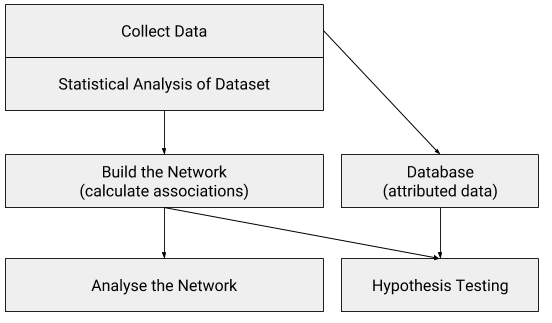
\includegraphics[width=1.0\textwidth]{Figures/WorkProcess}
	\caption{Steps of the Research Approach}
	\label{fig:process}
\end{figure}


\section{The Dataset}
\label{sec:dataset}
The basis of the dataset are video files, that capture tagged honey bees of one colony in a two sided observation hive.
Each individual of the colony, including about 3200 bees, were tagged with 12-bit markers. Four cameras were used to film the hive, the setup of the cameras is illustrated in figure~\ref{fig:cams} and an example of tagged bees is shown in figure~\ref{fig:markers}.

The recording season lastet nine weeks (63 days), around the clock, from 19.07.2016 until 19.09.2016, with some interruptions due to maintainance and technical failures, this is shown in figure~\ref{fig:period}. Those days were excluded completely.
The recording resolution of each camera is three frames per second, aiming for $1024$ frames (about $5.7$ minutes) for a video files.For each frame, bee detections were extracted by using an image analysis pipeline.

\begin{figure}[htb]
	\centering
	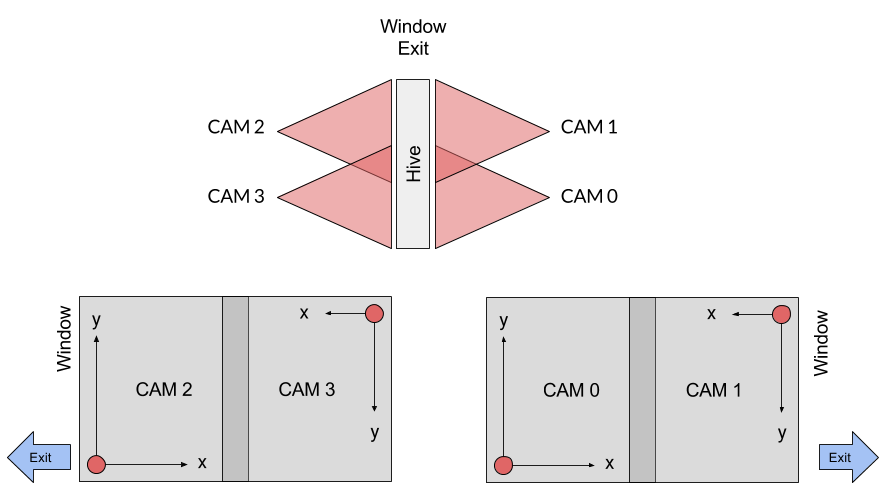
\includegraphics[width=1.0\textwidth]{Figures/setupCams}
	\caption{Camera Setup in 2016: (1) Top View:  vertical hive with two cameras for each side, overlapping in the middle. (2) Front View: left and right camera setup, the red dot indicated the origin $(0,0)$ of the camera.}
	\label{fig:cams}
\end{figure}

The resulting detection data is stored in a binary file format. A python library called \emph{bb-binary}\footnote{\url{https://github.com/BioroboticsLab/bb_binary}; Last accesed: 2106-02-16, 04:28PM} provides easy access to the binary files. Each file in bb\_binary file format corresponds to a video file of a single camera.
The size of the complete dataset for 2016 is $470$~GB, about $7.5$~GB of binary data per day.

Exactly $3.191$ bees were tagged. The tagging period is 67 days long. The tagging started on 2016-06-28 (22 days before the recording started) and lasted until 2016-09-02 (17 days before the recording ended). The young bees were tagged and then added to the hive, about noon each day. The overall tagging frequency is shown in figure~\ref{fig:tagging}. The hatching day for each bee is known, therefore the age of each bee.

\begin{figure}[htb]
	\centering
	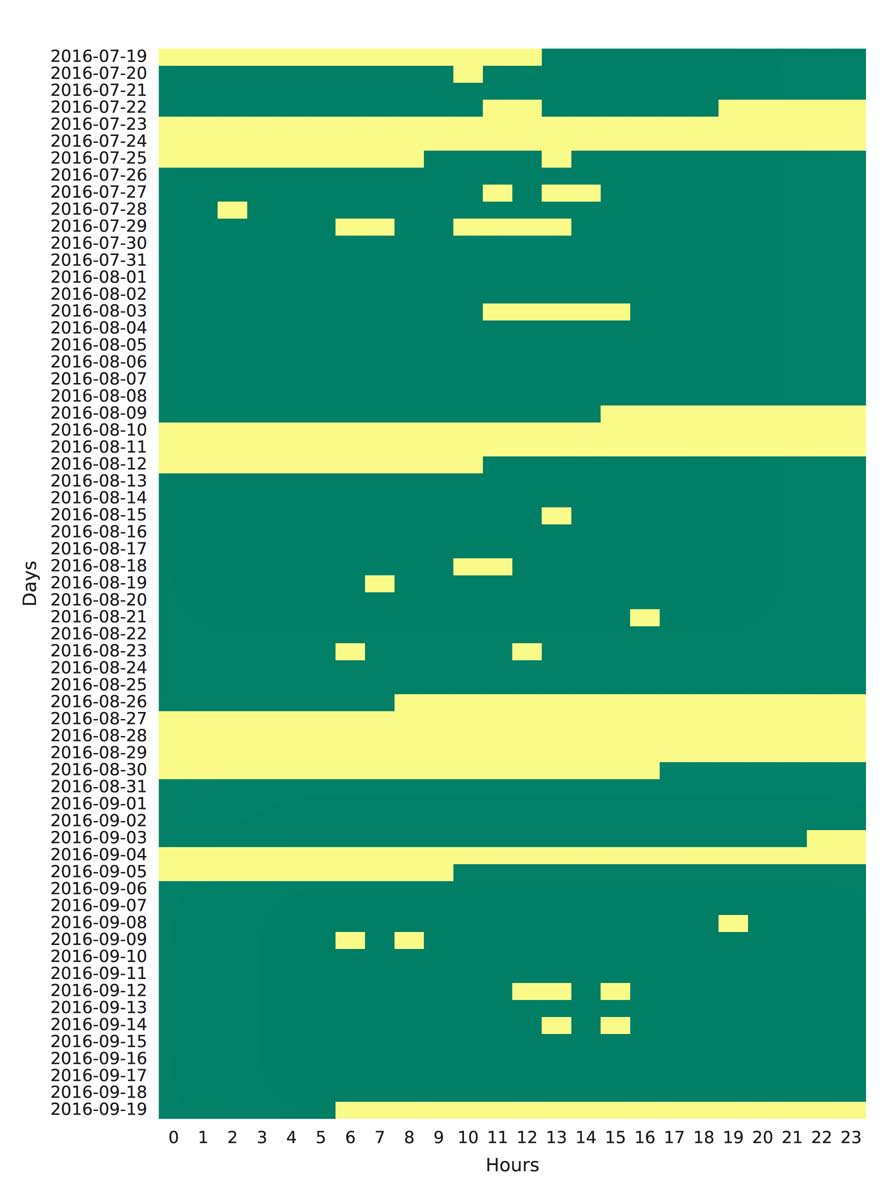
\includegraphics[width=1.0\textwidth]{Figures/recording}
	\caption[Recording Season with maintainance and failures]{Recording Season with maintainance and failures: \emph{Yellow} indicates recording went without any big interruption; \emph{Green} indicates maintainance work or technical failures of one or all cameras. This is calculated using the expected number of files produced by each camera per hour.}
	\label{fig:period}
\end{figure}

\begin{figure}[htb]
	\centering
	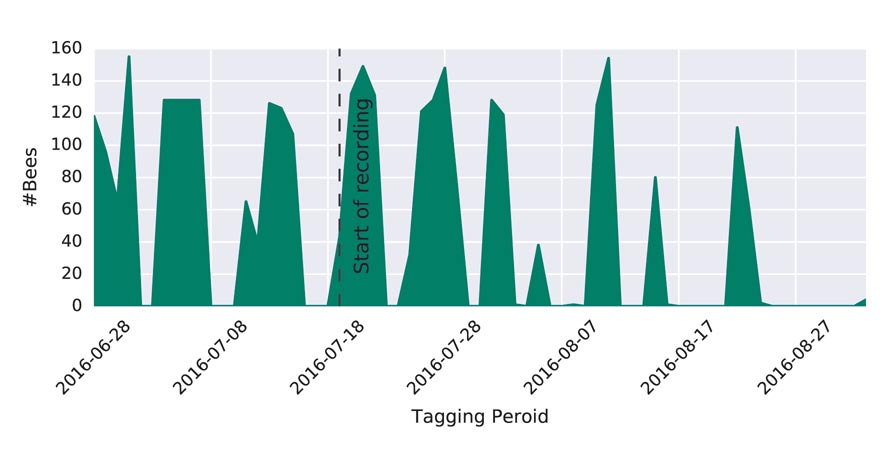
\includegraphics[width=1.0\textwidth]{Figures/tagging_period}
	\caption[Tagging Frequency]{Tagging frequency of bees: The bees were primarily tagged during the week. The weekend (sometimes also mondays or fridays) no bees were tagged. On average 48 bees were tagged each day, considering only tagging days, the average is about 91 ($\pm50$) bees (median 118, mode 128).}
	\label{fig:tagging}
\end{figure}

\subsection{Structure of the Dataset}
The data is organised in \emph{frame container}, wich corresponds to a video file of a single camera. A frame container holds all \emph{frames} for that specific video.
Each frame has a list of all bees detected by the image analysis pipeline.

A \emph{detection} has the following attributes, which are relevant to this project:

\begin{itemize}
\item \textbf{xpos}: $x$ coordinate of bee with respect to the image in pixel
\item \textbf{ypos}: $y$ coordinate of bee with respect to the image in pixel
\item \textbf{radius}: of the tag
\item \textbf{decodedId}: decoded 12-bit id, the bit probabilities are discretised to 0-255
\end{itemize}

Besides further information, the frame container specifies the camera and a frame is also attributed with a timestamp. The data can be accessed iterating on frame container or on frame level, in both cases using timestamps for start and end. The data scheme is illustrated in figure~\ref{fig:scheme}.
The complete data scheme can be found on github\footnote{\url{https://github.com/BioroboticsLab/bb_binary/blob/master/bb_binary/bb_binary_schema.capnp}; Last accessed: 2106-02-16, 04:46PM}. 


\subsection{Data Quality and ID Confidence}

Each bit of the decoded 12-bit ID represents a probability between $0$ and $255$. That means when using a high ID confidence\footnote{The confidence of an ID is calculated as follows. TODO. Each bit should be over the confidance value.} results in less data, but with a higher accuracy.
A low confidence results more data, but rather uncertaity and a higher error. A good tradeoff between data quality and amount of data should be chosen. Figure~\ref{fig:tradeoff} shows the proportion of wrong detections (as a fraction of all data) depending on the confidence level for all four cameras.

A confidence level of $0.95$ results in about $59\%$ of remaining data, of those about $6\%$ are wrong detections. This level of confidence is chosen.

Here should be some text about the tracking quality as well. For this confidence level I analysed the quality of the timeseries (tracking path) of a bee. The distribution of gap sizes of different length was used to measure the quality of the data. [TODO]

\begin{figure}[htb]
	\centering
	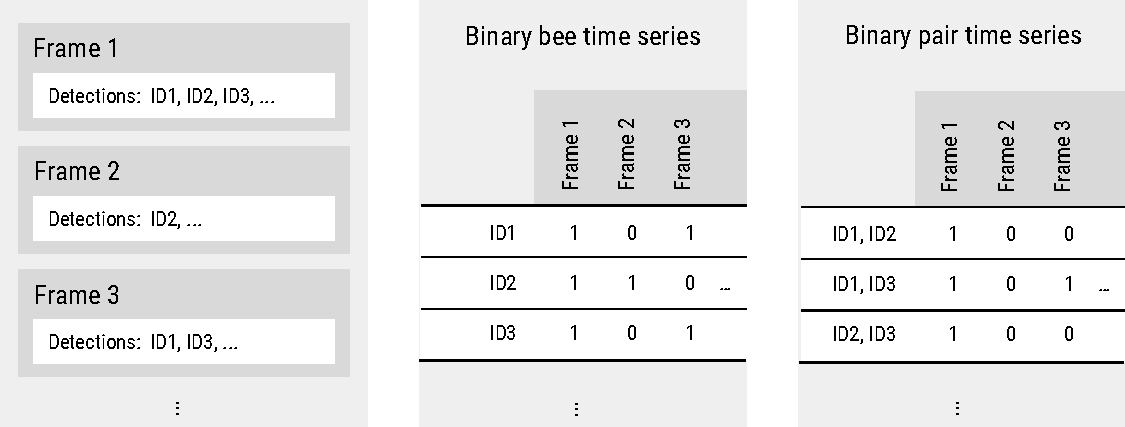
\includegraphics[width=1.0\textwidth]{Figures/structure}
	\caption{Structure of the data scheme}
	\label{fig:scheme}
\end{figure}

\begin{figure}[htb]
	\centering
	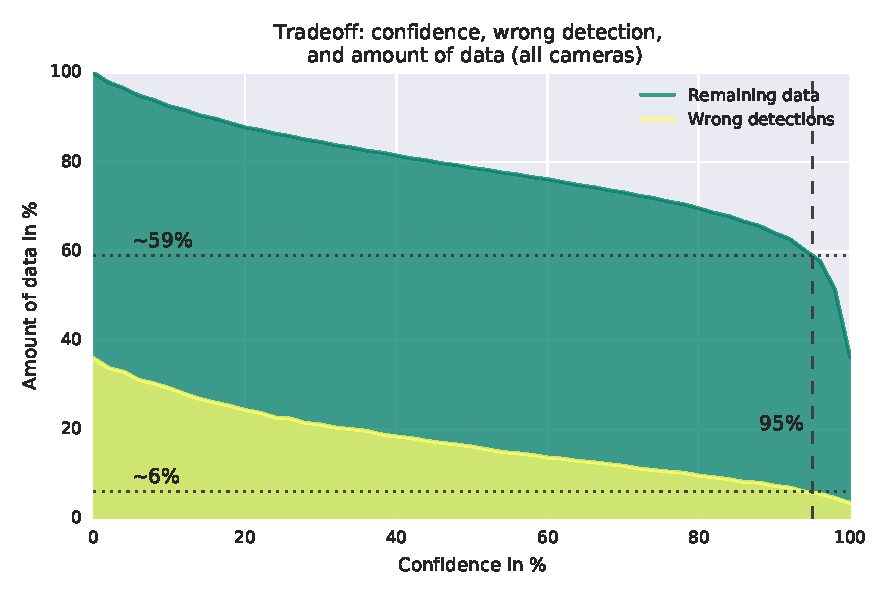
\includegraphics[width=1.0\textwidth]{Figures/tradeoff}
	\caption[Tradeoff: Confidence level, data quality and amount of data]{On 21.07.2016, about half of the bee tags were used up. This day was chosen to determine the effects of the ID confidence level on data quality and amount of remaining data. For each camera a five minute test dataset was chosen (15:00-15:5). For a sample ($n= 100.000$) of remaining detection, the age was determined, negative ages were counted as wrong detections (times two).}
	\label{fig:tradeoff}
\end{figure}


\subsection{Statistical Description of the Dataset}
i will fill this part, when I need it\\
speed of bees\\
presence and absence of bees (counted and as duration)\\
presence and absence of bee-pairs (counted and as duration)\\
number of detected bees per day (and hour)\\ 
not sure if so much is needed\\
will see later\\


\subsection{Implications}
only some days can be used for creating the networks , due to technical problems\\
confidence $95\%$\\
the absence of bees can have a lot of reasons, beeing inside a cell, outside the hive, ID quality to bad (confidence), not detected by camera because inside the exit, backwards on the window pane, difficult angle of tag, coverd by another bee, and so on an ond.\\
Therefore the detection of bees, who are close to each other (who are likely to interact), should be not that strict, or at least variable.\\


\section{Inferring Networks}

The following part describes the pipeline for generating spatial proximity networks out of honey bee tracking data. A node in the network is a bee. They are distinguished by IDs. Two bees are associated if they have a maximum distance, $d$ (distance) for at least $f$ frames (1 frame = 0.33 second). This is stupid, as there are gaps which result from detection errors or confidence.

contact rate and contact duration\\

\subsection{Network Pipeline}
\subsection{Thresholding Edges}

\section{Static and Temporal Analysis}	

\section{Attributed Data and Hypothesis Testing}


\section{Implementation, Runtime and Complexity}
For implementing the network pipeline python, with pandas and numpy, are used, because the bb\_binary library, for accessing the tracking, data is only available in python. The networks, in graphML format, are created using the python library \emph{NetworkX}\footnote{\url{https://networkx.github.io/} ; Last accessed: 2017-02-17, 08:07PM} in version 1.11.
iGraph for community detection\\
some bash scrips for generating multiple networks\\

bottleneck is reading bb\_binary data into pandas dataframes\\
using multithreading for distribution on frame level (a process gets X frames for processing)\\

maybe some table with how long nees what with how many cores\\

